\section{Preliminary Results}
\frame{Preliminary Results}

\begin{frame}{Tracking Trajectory}
\begin{itemize}
    \item Let $\gamma : t \rightarrow \phi(t;x_0, u^\theta)$ represent the flow of the dynamical system.
    \item The objective is to learn a closed-loop controller that tracks an expert trajectory $\gamma^\star$ provided by a path planner.
    \item The running cost that achieves this is given by 
    \begin{align*}
        J_{track}(\gamma, \gamma^\star) &= \sum_{i} |\left| \gamma_{i} - \gamma^\star_{i} | \right |^2.
    \end{align*}
    % where $(\cdot)_\bot$ expresses the state in transverse coordinates along the desired orbit $\gamma^\star$.
    \item The performance of NBL is tested on the swing-up task of the simple pendulum.
\end{itemize}
\end{frame}

\begin{frame}
    \small
    \begin{columns}
        \begin{column}{0.4\linewidth}
            \begin{itemize}
                \item The stochastic policy is marginalized over the posterior: 
                \begin{align*}
                    u(x) = \frac{1}{N}\sum_{\theta \sim q(\theta; z)} \mathcal{D}\{F(x; \theta) \}.
                \end{align*}
                \item Deterministic and stochastic policies are compared against
                system parameter and measurement uncertainties.
                \item Measurement noise on position $\epsilon_q= 0.0005$ radians, and velocity $\epsilon_{\dot{q}}= 0.05$ radians/s.
                % \item The continuous error band is generated by computed accumulated loss over 20 trajectories.
            \end{itemize}
        \end{column}
        \begin{column}{0.6\linewidth}
            \begin{figure}
                \centering
                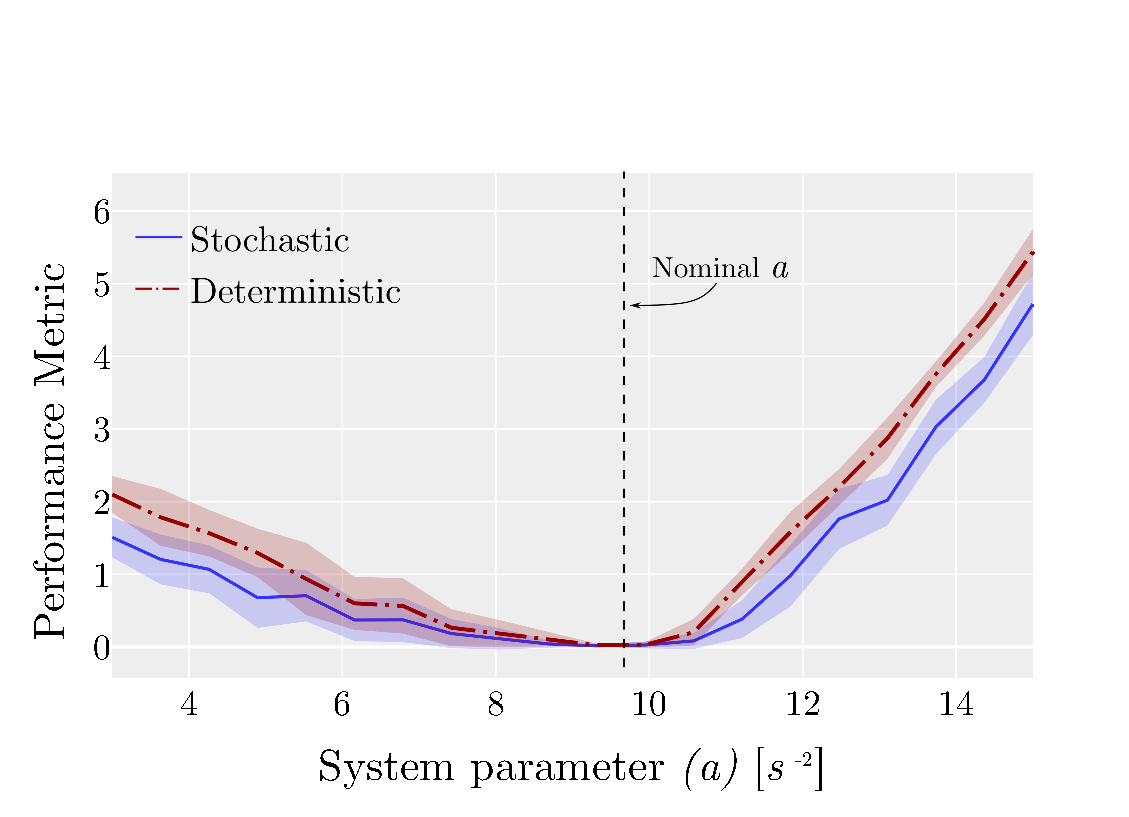
\includegraphics[width=1.0\linewidth]{figures/H.eps}
                \caption{\small Performance metric is the minimum loss to the expert trajectory over the last 2 seconds of a 10-second-long trajectory}
            \end{figure}
        \end{column}
    \end{columns}
\end{frame}

\begin{frame}{\textsc{IdaPbc} on the Inertia Wheel Pendulum: Simulation Tests}
    \begin{columns}
        \begin{column}{0.48\linewidth}
            \small
            \begin{itemize}
                \item The objective is to use the momentum from the wheel to swing up the pendulum.
                \item The dynamics of the system under measurement noise is 

            \begin{equation*}
                \dd x = \bmat{\dot{q}_1 \\ \dot{q}_2 \\ \dfrac{mgl \sin(q_1) - u^\theta - b_1\dot{q}_1}{I_1} \\ \dfrac{u^\theta - b_2 \dot{q}_2}{I_2}} \dd t + \nabla_x u^\theta(x) \sigma \dd W_t
            \end{equation*}
            \item Performance metric is $\int_0^T \left(\frac{1}{2}qx^2 + \frac{1}{2}ru^2 \right) dt$.
        \end{itemize}
        \end{column}
        \begin{column}{0.52\linewidth}
            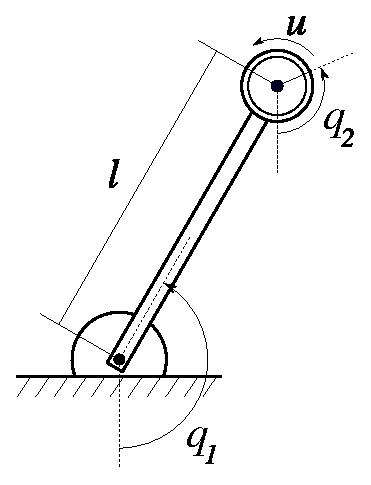
\includegraphics[width=0.25\linewidth, center]{figures/iwp.eps}
            \vspace{-0.95cm}
            \begin{figure}
                \centering
                \includegraphics[width=0.9\linewidth, center]{figures/bandplot1.eps}
                % \caption{Performance metric is accumulated quadratic cost}
            \end{figure}
        \end{column}
    \end{columns}
\end{frame}


\begin{frame}{\textsc{IdaPbc} on the Inertia Wheel Pendulum: Experiments}
    \begin{columns}[c]
        \begin{column}{0.5\linewidth}
            \begin{itemize}
                \item The mass of the wheel is varied according to Table 1.
                \item The same controller is tested on various system parameters.
            \end{itemize}
            \begin{table}
                \centering
                \footnotesize
                \caption{System parameters used in real-world experiments. The errors in the
                last column are $\|\zeta - \zeta_0\| / \|\zeta_0\|$}.
                % \rowcolors{2}{}{Wheat1}
                \begin{tabular}{lcccc}
                  \toprule
                  Parameter set $\zeta$ & $I_1$ & $I_2$ & $mgl$ & Error \\
                  \midrule
                  Nominal & 0.0455 & 0.00425 & 1.795 & 0 \\
                  3 Rings & 0.0417 & 0.00330 & 1.577 & $0.122$ \\
                  2 Rings & 0.0378 & 0.00235 & 1.358 & $0.243$ \\
                  1 Ring & 0.0340 & 0.00141 & 1.140 & $0.365$ \\
                  \bottomrule
                \end{tabular}
                \label{tab:modified_params}
              \end{table}
        \end{column}
        \begin{column}{0.5\linewidth}
            \includegraphics[width=0.6\linewidth, center]{figures/4_rings_Moment (2).jpg}
            \begin{figure}
                \centering
                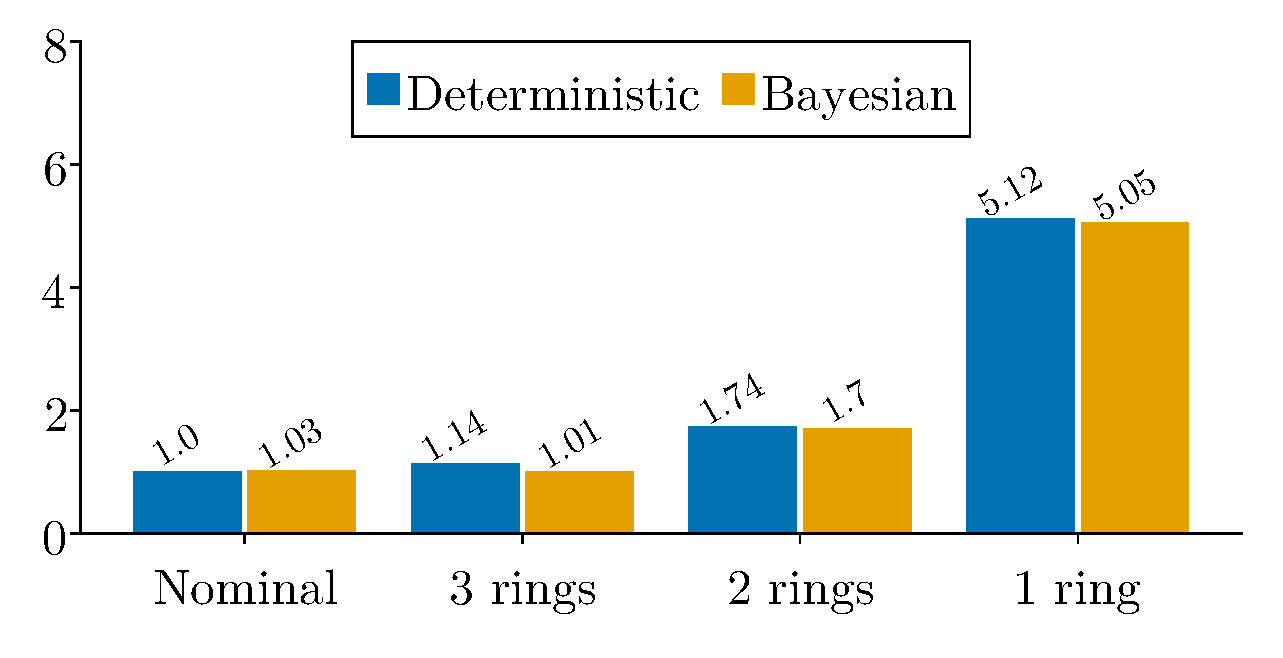
\includegraphics[width=0.8\linewidth, center]{figures/idapbc_bar.eps}
                \caption{\small Performance metric is $\int_0^T \left(\frac{1}{2}qx^2 + \frac{1}{2}ru^2 \right) dt$}
            \end{figure}
        \end{column}
    \end{columns}
\end{frame}

